% Chapter 6

\chapter{Final version} % Main chapter title

\label{Chapter6} % For referencing the chapter elsewhere, use \ref{Chapter5} 

Here will be explained the features of the final version, and how we are arrived at it. This version is very near to what we want to create as definitive application.

\section{Functional requirements}

The last version (from now "gAn Web v3") is a modified version of the intermediate version. 
The second version's modifications come from two sources: some adding requirements and modifications are proposed from the super users and some else come from the tests made with the generic users; 
The first group of adding requirements (the ones proposed by the supervisors) are the following:

\begin{enumerate}
%1 choose analysis new way
\item 
The main kinds of analysis are now more clear: they are around 10, and they are     quite stable (their goals, so their input and expected output are quite stable, but still we'll probably modify the algorithmic ways in which these goals are achieved; from the point of view of the web interface the situation is quite stable). Their roles and when they are useful is now steadily fixed (more precisely: we are pretty sure about the role of the existing analysis, but in the future we can add more analysis..). Each user, according on his task, knows (should know) in every moment which analysis fits better the situation, so, the best solution is to allow the user to choose the type of the analysis through a dropdown menu directly in the main page (exactly like he chooses the run number). To make the user's life easier the application can use a tooltip for each analysis, to remember him in which situation it is useful. At this point the possibility of choose the gAn version is useless, because the definitive version of gAn include all the existing types of analysis. 

%2 single vs multiple
\item 
The kind of use of this software is quite different if you decide to work with a single run or a group of runs, so is better if at the beginning (at the application starting) the user chooses directly if he wants work with a single run or more than one. 

So the application becomes modal: it can be a problem and can create confusion, but we hope that the simplicity of the interaction and the presence of a box that constantly informs the user about which "mode" he is using can reduce confusion instead of let it grow.  

If the user works with a single run the focus is mainly on the "exploration" of the information in the data, with the multiple runs the focus is more on the possibility to compare and see what is different.

In the second case (more than one) is better to tell if the runs are a range (from N to M, all the runs between) or a group of non-consecutive runs (it can be useful, because of the feasibility to compare non-consecutive runs can be interesting). If the user is interested in a group of runs that are not a range (we observe that this situation is not common, but we must manage it), the previous solution of multiple runs separated by a comma is not a good idea: often in these cases the researched runs are little consecutive groups, so a list of ranges. It is better if the user can have an input area (like a sheet) in which he can put the intervals, divided in different lines (or other separators).

%3 don't choose root version
\item
There is an effort in the developing of the whole project to make it independent of the Root version, so the interface won't ask to the user to choose a Root version anymore. 

%4 need to be quite aesthetically acceptable
\item
The aesthetic part in this application was neglected in the first and intermediate versions, but now it needs to be cured and improved to ensure the best possible satisfaction to the users. 

\end{enumerate}
 
Furthermore, the version with this last requirements was tested with the users: the developer studied their behavior observing them at work with the existing version, listening to their comments, and asking them opinion. The impact of the debut with the users highlights some problems to be overcome, and also provide some interesting ideas: from the analysis and the solution of these problems and from the user's proposals the requirements of the last version was defined. 

In this document there is a chapter (\ref{Chapter6} ) aimed to explain how the tests with the users took place and what are the results, to know more about the argument.

The main problems observed (and for each the proposed solution) are the following:

\begin{enumerate}
\item 
It is important to help the user in some way to choose the run number: the user needs a view on the logbook of the run, that is a text in which there are information about each run number grouped by date.

\item
Actually nobody use the button to modify the dimension of the images: they all use the biggest version.. is better to remove (or move in a less central place) this dropdown menu. A similar reasoning can be done for the dropdown that allows the user to switch between the vertical and carousel menu (everybody use vertical, clearly at this point the carousel version isn't useful). Also nobody use the run selector to choose which image see: they prefer base themselves on the image's title.. at this point a surely better recognize that the existing navbar is not suitable to satisfy the needs of the user, a better solution is to create a selector with the image's titles, precisely a group of check-boxes, each with the title of an image as label, using that the user can select one or more (or all if he wants) images.  

\item
The read of the textual output takes too much time: it can be improved highlighting the most important parts (or better, the most important parts for the selected type of analysis)

\item
The user needs to choose by the configuration page the degree of precision (the minimal error) of the x-axis (the time related axis) of each time-related values images. This parameter seemed to be not very important and in the second version actually there wasn't, but almost all the users modify it quite often (manually), and verbally ask for the possibility to set it through the interface. So is better to let them to do it by the interface

\item
The general organization of the output is simply not the best possible: the users need to switch easily from textual to images output and vice-versa, and the buttons are too many spread on the screen, so too difficult to find.

\end{enumerate}

\section{Non-functional requirements}

There is another special requirement emerged in this version, not strictly related to the common behavior of the interface but quite important: the machine  used as server is also used for the testing of single analysis when they are written; sometimes these analysis crashes (quite normal in a test phase), and they remain in a "hung up" state, without doing nothing but occupying Ram memory, and if the blocked application are numerous that can be a problem for the performances of the machine. To ensure a correct behavior gAn Web must check this situation at starting and eventually resolve it.

\section{Scenario based functional analysis}
Following we can show some examples able to explain how the typical interaction must work in the definitive version:

\begin{enumerate}

\item
Let's suppose a very common situation in a shift: 
In the shift is running the run NNNN. The shifter wants to calculate the temperature of some particles with a (complex) process based on the shape that they create on a sensor (the basic idea is: if a particle is hotter, its speed is bigger, it can escape more easily from a magnetic trap, and the sensor can observe more particles outside the trap. At this point the software tries to fit, with an exponential function, the shape of the signal that the sensor shows as output, and through the integral of the slope of this exponential function can estimate the temperature of the particle).
The user chooses the single analysis, inserts the run NNNN, selects the kind of analysis called "TemperatureMeasurement", clicks the "start" button;
The system shows to the user a textual output and some images: 
The textual output proposes a lot of information, but in the ninety five per cent of the cases the user is interested in only three parameters, that are clearly highlighted by a special font, a color and a visible border. 

The user must also check the image: there is the histogram of a signal, an a red line where the function is fitted. The user checks if the red line
has an exponential shape (if it is a straight line the situation is too aleatory and the data are not affordable); the user also checks if the fit line is too long (it must be very little to accept the results of the analysis, because of physical reasons). 

Let's suppose that the fit function is a straight line: the user can retry the same analysis with a different setting: he returns to the homepage (through the button "New Analysis" on the Navbar), he clicks "Advanced Settings" to modify the configuration, he inserts a new value through a slider, to have a more precise graph, in the hope to fit it better. At this point he can retry the previous algorithm (a more precise function will lead a slower computation but probably will give an affordable output)  

\item 
The user is interested in a two distinguished groups of runs, from 57001 to 57005 and form 57016-57020.
This situation is very common because most of the groups of measurements are repeated in two different slices of times (to be sure about the results).
In this case the user, after having selected "Multiple runs", can click on "By InputArea" and a text area appears. In the area there are the value inserted the last time that the user used this function (we observe that is quite common repeat analyses with the same groups). The input is quite free: user can insert a group inserting the first and the last separated by a dash, a space, or a comma, and other group by changing the line (so each not empty line is a group). 
The user at this point selects the analysis and run the program. 

\item
The user is interested in a range of runs, from 58001 to 58010, to perform the same analysis and check if and how some values are varying. He can select multiple runs, insert the first and the last, select the analysis (the multiple runs analysis are taken from a different set from the single runs analysis).

\item
The user inserts a run, and selects an analysis names PMTs. This kind of analysis takes information from a group of sensors and produces in output (usually) seven images. The user often is not interested in all the seven images but in one or two. At this point, using the check-boxes selector he can select/deselect images to show (by default they are all selected).  

\end{enumerate}

\newpage
\section{Prototyping - Implementation}

Here is explained with some screen-shots how the final version looks like, and how does it work.

Login page:


\begin{figure}[H]
\centering
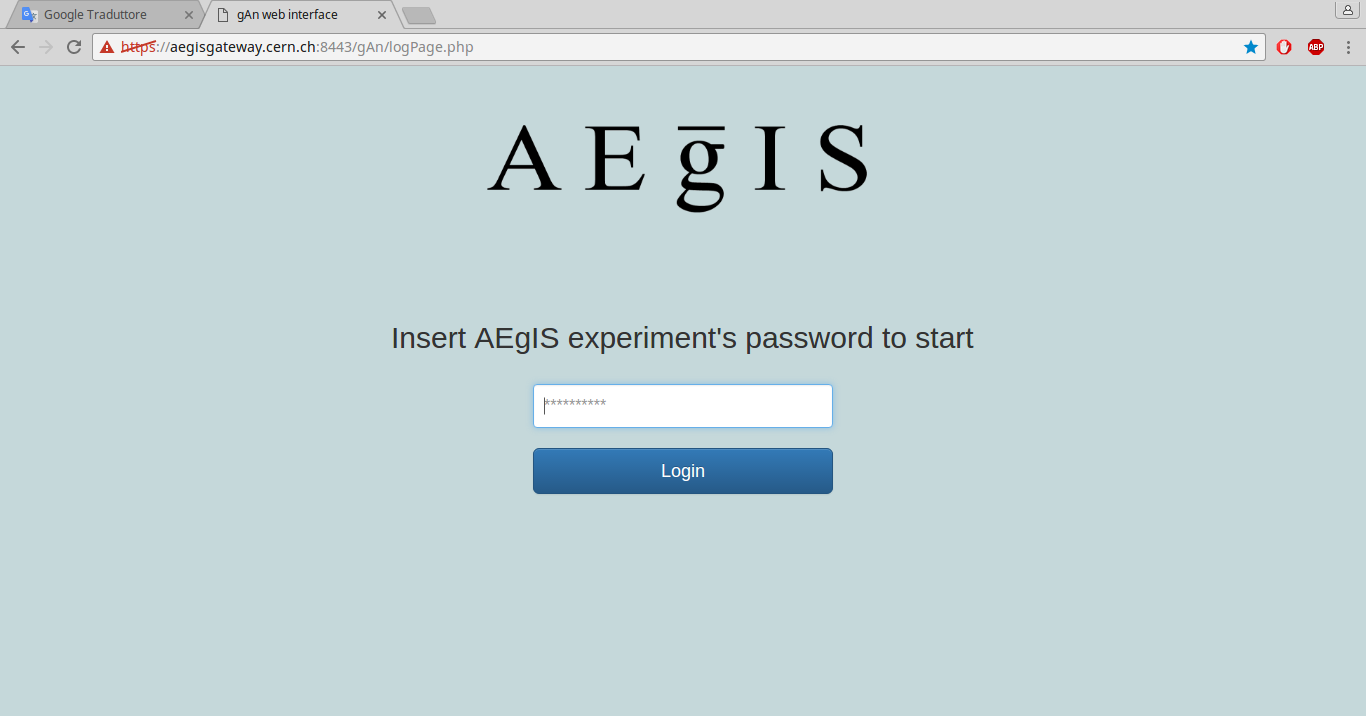
\includegraphics[scale=0.25]{LastLogin.png} 
\caption{Final version: the Login Page of gAn Web}
\end{figure}

First of all the login page: it is very simple, only one user exists (all the people in the AEgIS experiment are equal when they use this software, and no others experiments use this application) so only the password needs to be inserted, in order to ensure that only people who work in the experiment can use the software. We can see the typical objects taken from the Bootstrap's default graphic objects.

\newpage

Home page, initial choice:

\begin{figure}[H]
\centering
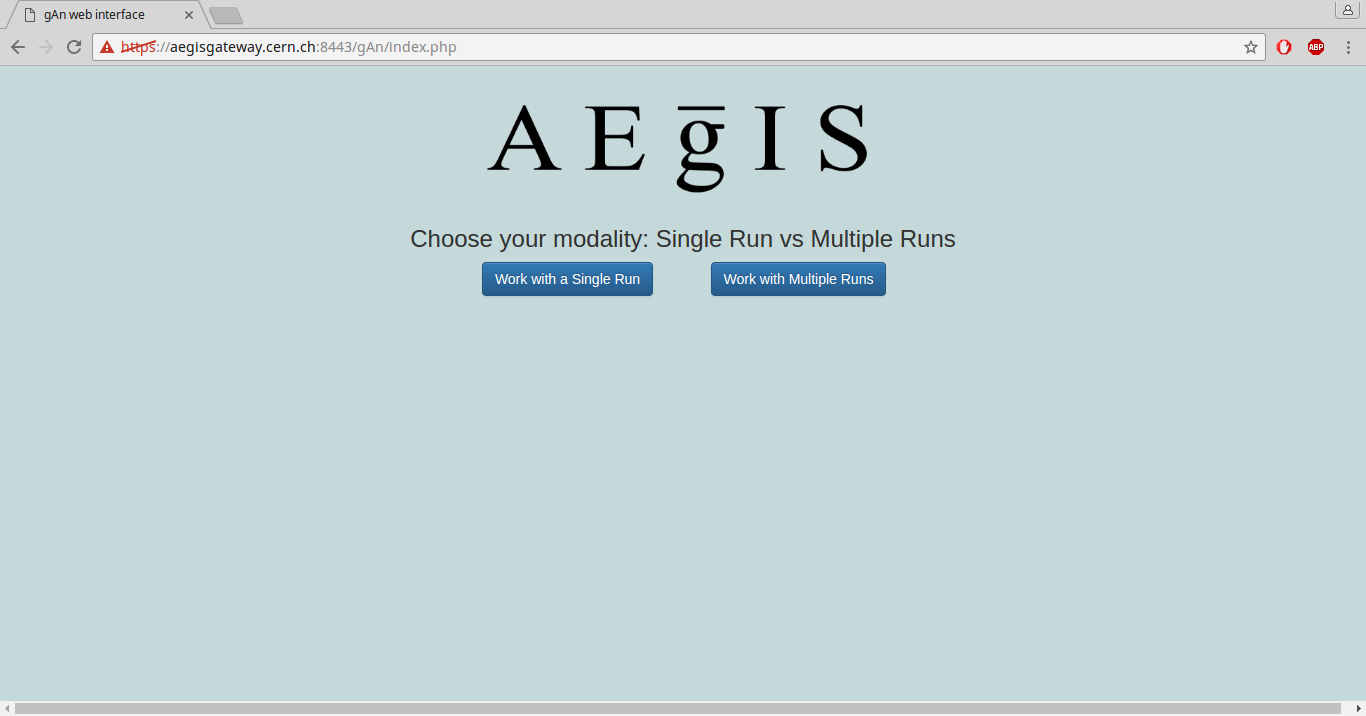
\includegraphics[scale=0.25]{LastInitialChoice.png} 
\caption{Final version: the first thing that a logged user sees}
\end{figure}
  
The neo-logged user can here choose if he is interested in a single run analysis of in a multiple runs one. These two situations are quite different, so the application works with them in two different ways.

After the choice, the user can always change idea, by the appropriate button:

\begin{figure}[H]
\centering

\includegraphics[scale=0.25]{ParticularExitStrategy.png} 
\caption{Final version: how the user can change his choice}
\end{figure}

\newpage
Home page, differences between single and multiple runs:

Here we can see how the two modalities of work (single and multiple) appear.

Single run: 
\begin{figure}[H]
\centering
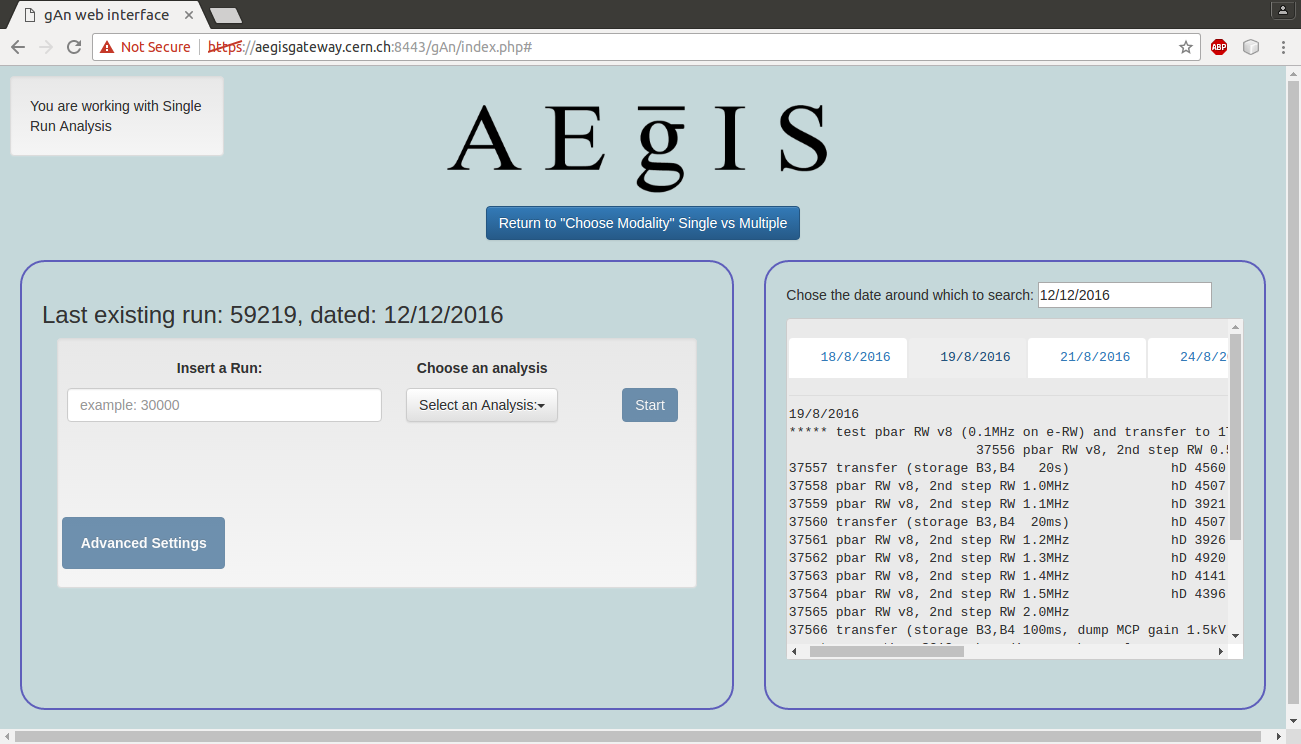
\includegraphics[scale=0.25]{LastSingle.png} 
\caption{Final version: the Homepage if the user chooses Single run analysis}
\end{figure}

the single one is more simple, on the left of the screen the user inserts a run number and a kind of analysis. We can see the button related to access the configuration page and modify the settings (Advanced Settings). On the right part of the screen there is a view on the RunLog of the experiment. The user uses the right part when he wants more information about what run use to work (actually this situation is quite seldom). In the case the user can insert a date using a datepicker, the system opens some pages related to the days around that date and in each page shows the content of the logs related to this date. The goal of the datepicker, provided by Bootstrap, is to reduce the charge on the memory of the users (it shows as default the current date, and shows as result the pages of the RunLog related not only to the selected date but also to the days before and after, to give the user some references and allow him to make errors of 2-3 days still finding the result) and to allow him to insert the date in a correct format. The logs are always divided in runs, and for each run there are some information and comments. At the moment this functionality is a mock-up (it is one of the few  mock-ups exposed in this document). 

On the top-left of the screen there is always a little note with some information about the status of the program: this is a little cognitive aid:


\begin{figure}[H]
\centering
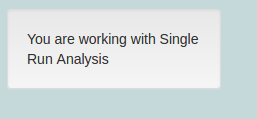
\includegraphics[scale=0.45]{ParticularStatusHP.png} 
\caption{Final version: a label with some information about the current status is always visible in the homepage}
\end{figure}    
 


On the screen there is always written the last known run, because in most cases the users use it or the immediately previous one. 

The interface informs the user if he makes some errors inserting the input. On the first implementation the error messages was programmed to became visible every time the inserted value was incorrect, so also at the moment the user was entering in the page and still hasn't inserted the values. This behavior is quite aggressive and unkind to the user.. it is surely not our intention so is a better solution if the error messages appear only when the user try to click send without having inserted correct values. The messages are hopefully aimed to explain the user how to solve the problem:

\begin{figure}[H]
\centering
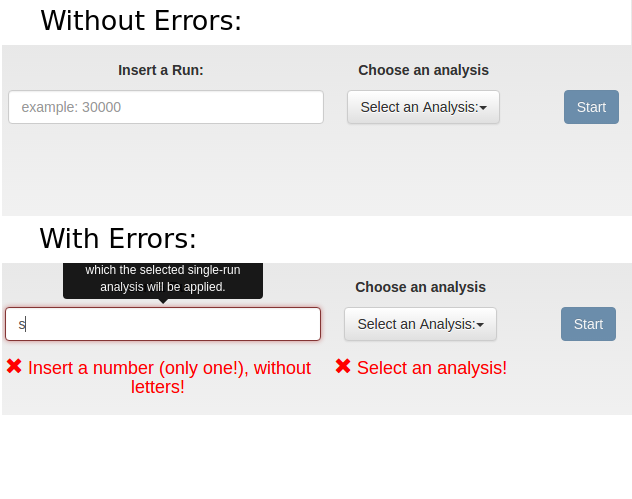
\includegraphics[scale=0.5]{ParticularHowErrorsWork.png} 
\caption{Final version: how error messages work}
\end{figure}    


\newpage
The dropdown menu usable to choose the kind of analysis is quite long (up to 10 options). A good idea is to order it and organize it in homogeneous groups:

\begin{figure}[H]
\centering
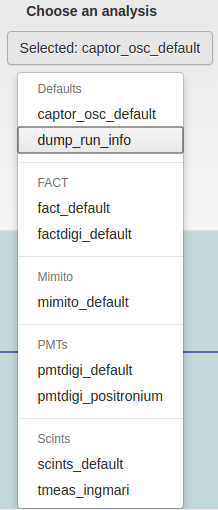
\includegraphics[scale=0.5]{ParticularDropDownSpecial.png} 
\caption{Final version: grouped dropdown menu}
\end{figure}    

  
Multiple runs:  
There is two different ideas about how to implement this page, because the new requisite about the fact that now the user can choose if insert one or more range using two input fields (for the first and for the last run) or a more flexible (but less efficient) "text area" is different from the previous version . So two different solution are evaluated, for convenience in this paragraph they are called "first" and "second", where the second is the correction of the first. So the first one was used to understand if the functionality is useful, the second one is a correction to ensure a more clear and better organized interface. At the end the second is the only one adopted in the application.

\newpage

Multiple runs first version:
\begin{figure}[H]
\centering
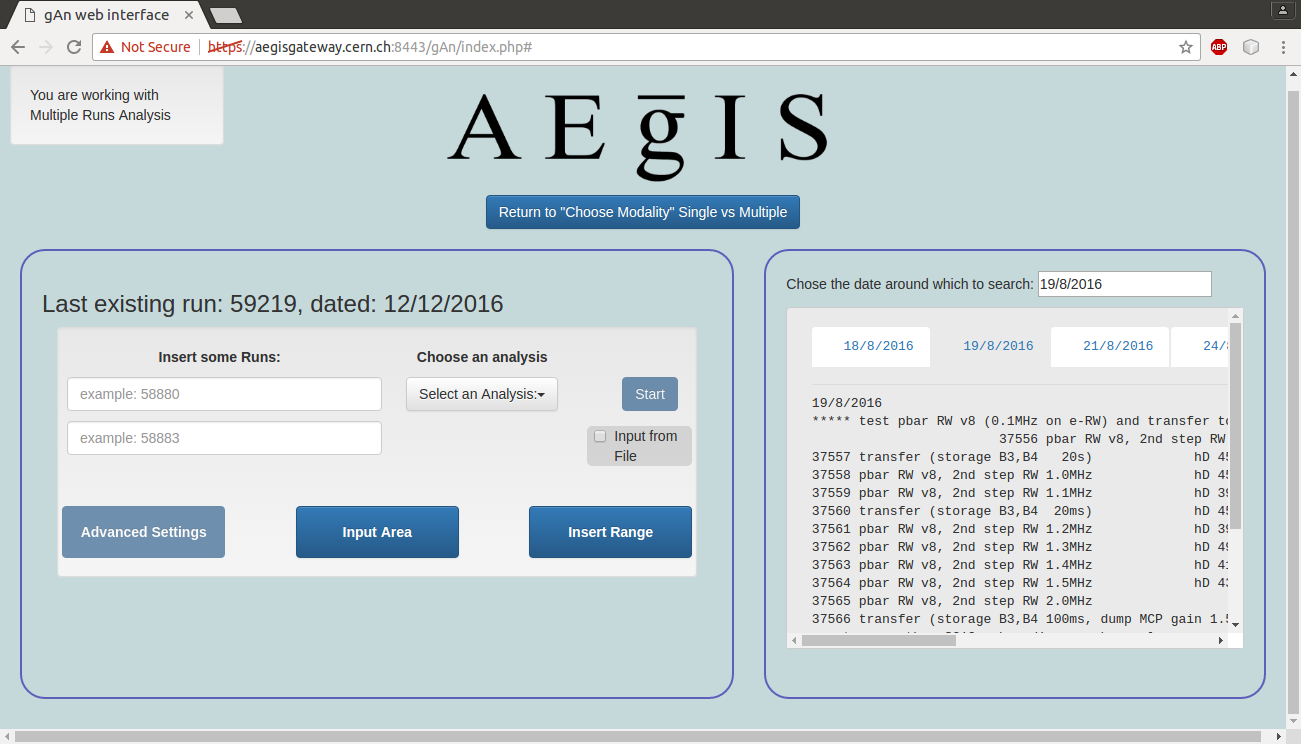
\includegraphics[scale=0.25]{LastMultipleFirst.png} 
\caption{Final version: the Homepage if the user chooses multiple runs analysis (first implementation)}
\end{figure}    

The multiple runs modality is similar to the single run but more complex: in a standard situation the user inserts two runs, the first and the last. The alternative (less used) situation is the one in which the user, through the "Input Area" button inserts a list of groups of runs (these runs are written in a file, that the system is able to accept as input). This modality is sometimes useful, and can be activated with the check-box "Input from file". The activation of this modality denies the access to the two input fields (you must only one way to insert runs..).
Following a little example of how the user can insert data through an Input Area in the first version:

\begin{figure}[H]
\centering
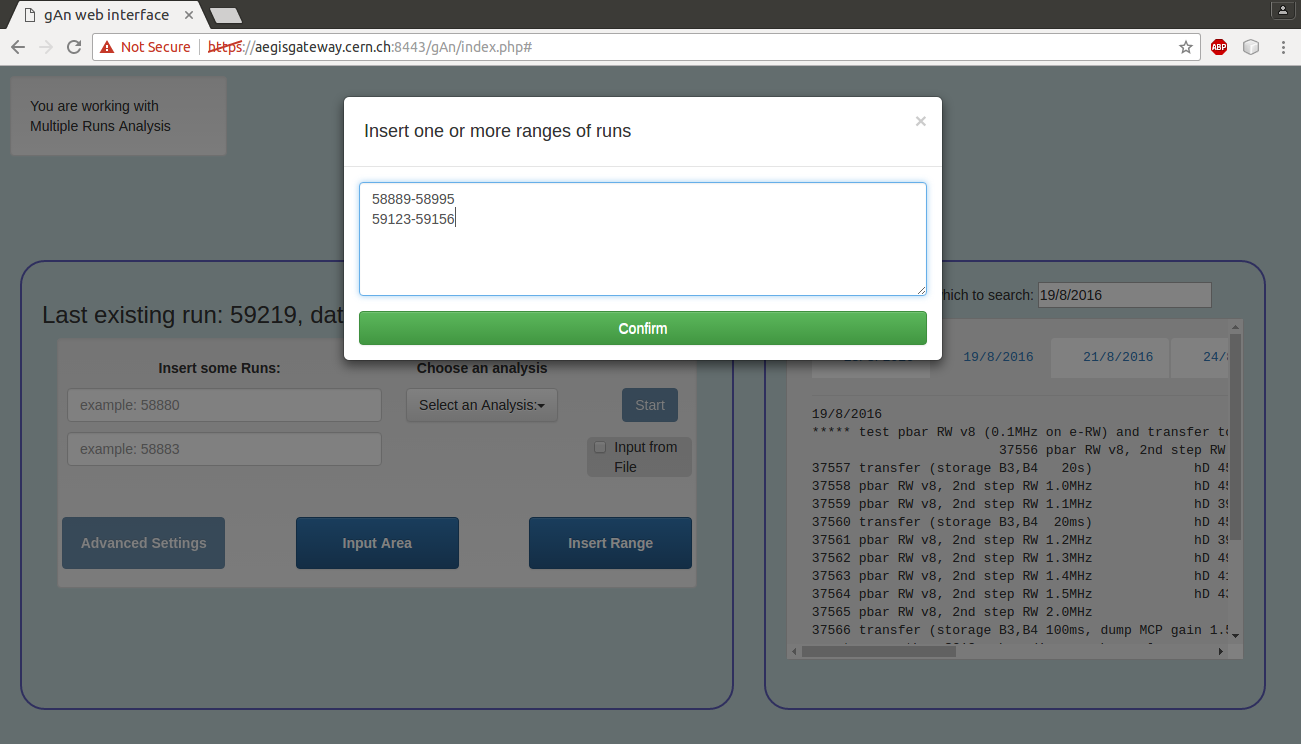
\includegraphics[scale=0.25]{LastMultipleRange.png} 
\caption{Final version: modal using which the users insert different ranges of runs (first implementation)}
\end{figure}   

Multiple runs second version:
The differences are only related to "how" the users can access the input field and the text area, the back-end is the same. Now the user can through a switching selector select which way he wants use to insert the runs. Obviously the selection of one way hides momentary the other one:

\begin{figure}[H]
\centering
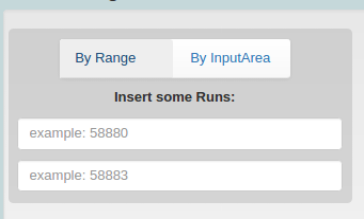
\includegraphics[scale=0.25]{ParticularRange.png} 
\caption{Final version: here is if the user selects "By Range" (second implementation)}
\end{figure}   

\begin{figure}[H]
\centering
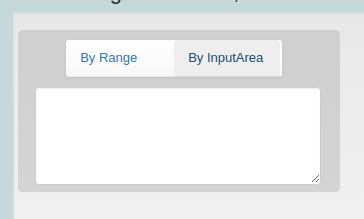
\includegraphics[scale=0.25]{ParticularInputArea.png} 
\caption{Final version: here is if the user selects "By InputArea" (second implementation)}
\end{figure}   

Now the little check-box near the start button is no-more useful (actually it created confusion), like the "Input Area" button. The interface is now more clear, without modals, with fewer commands but able to do the same things. A well surrounds the "runs related" part of the input system that now is quite composed and needs to be perceived like a "group".
Following how the multiple-runs interface appears now:

\begin{figure}[H]
\centering
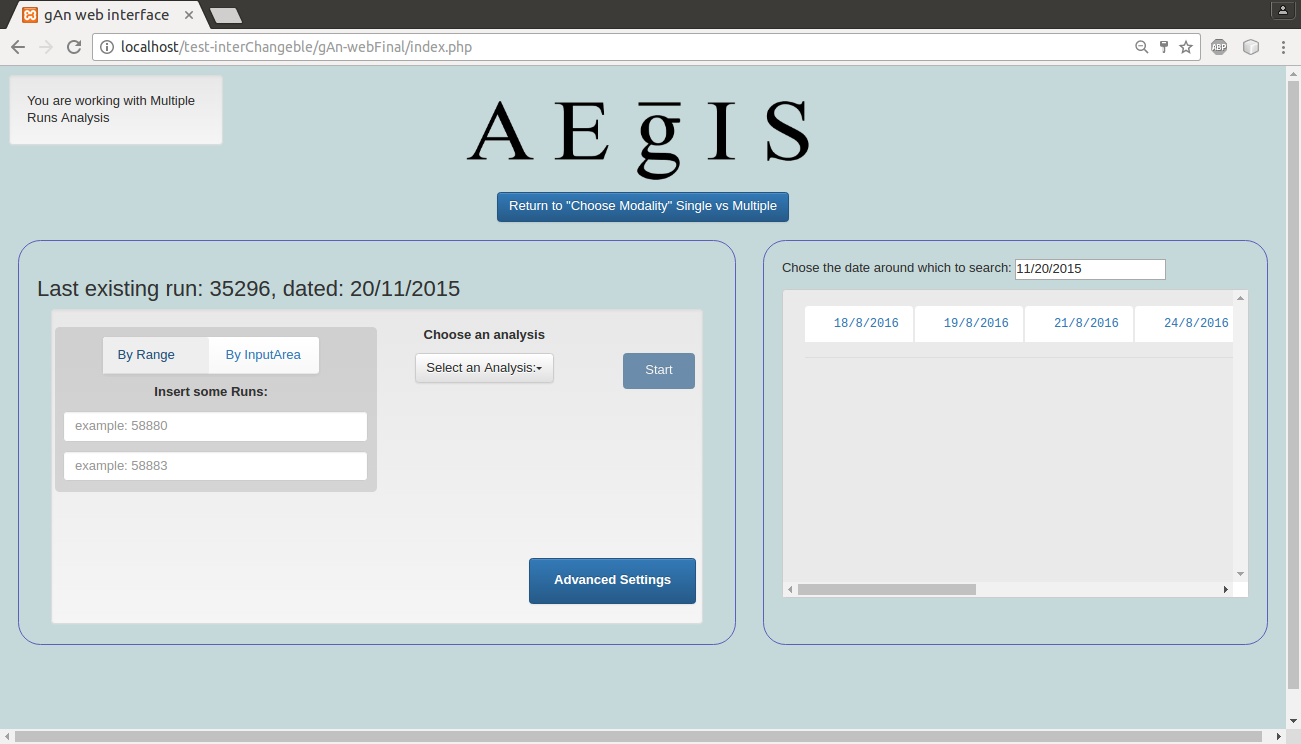
\includegraphics[scale=0.35]{LastMultipleSecond.png} 
\caption{Final version: how the homepage appears (second implementation)}
\end{figure}  

Advanced Settings page:

\begin{figure}[H]
\centering
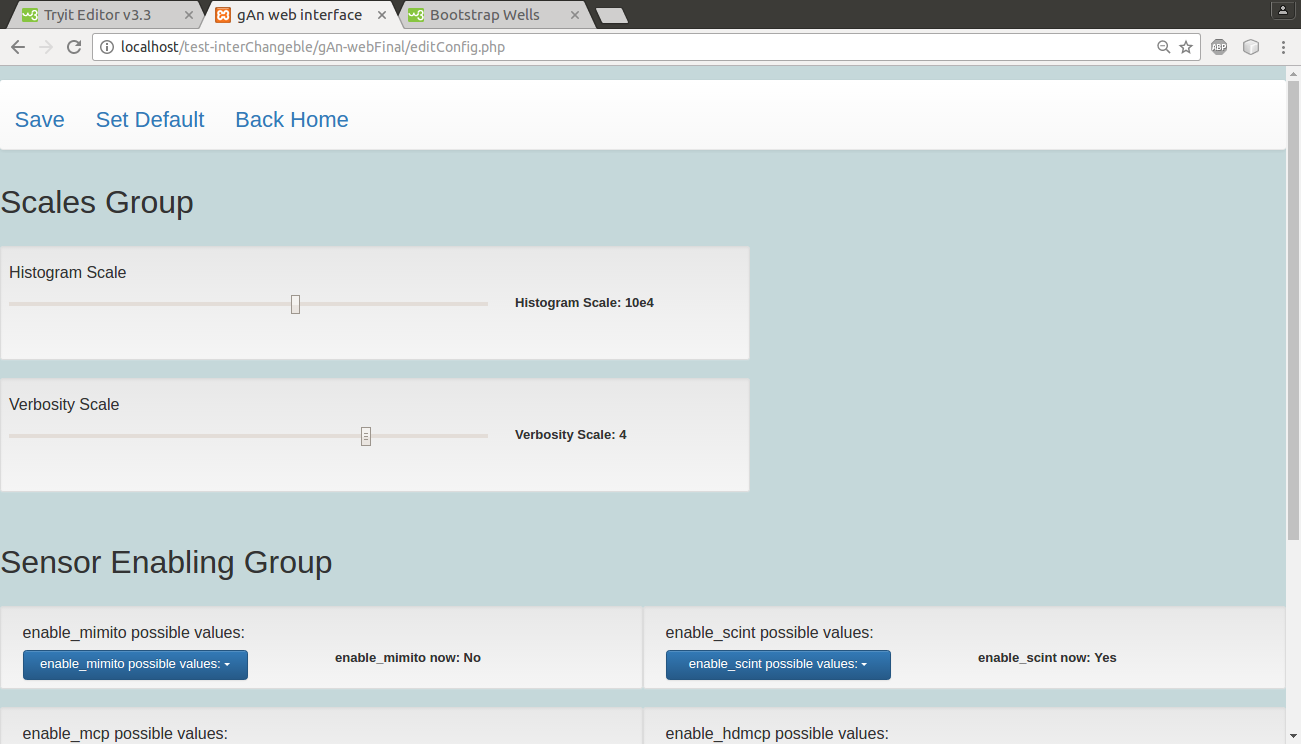
\includegraphics[scale=0.25]{LastEditConfig.png} 
\caption{Final version: the page related to edit configurations}
\end{figure}   

This page aims to allow the user to modify some groups of settings. The general rule is to use dropdown menus if the choice is true/false or Yes/No (	quite common) or between a reduced number of textual options, an to use instead  seekbars (an input bar moving which the user can insert a bigger or smaller numerical value) when the user must set a numerical value that goes from a minimum to a maximum value. On the top of the screen the user chooses to save the current setting, to return to the default setting, to go back home (without saving).    

In some cases the values to insert by the seekbars are in a very big range and is not easy to the user to have a too long seekbar. A good solution is to choose an exponential values seekbar: so the user chooses the exponentiation, not the number. This choice is quite reckless for normal users.. but for physicists the understanding of how an exponential value works is not a problem:

\begin{figure}[H]
\centering
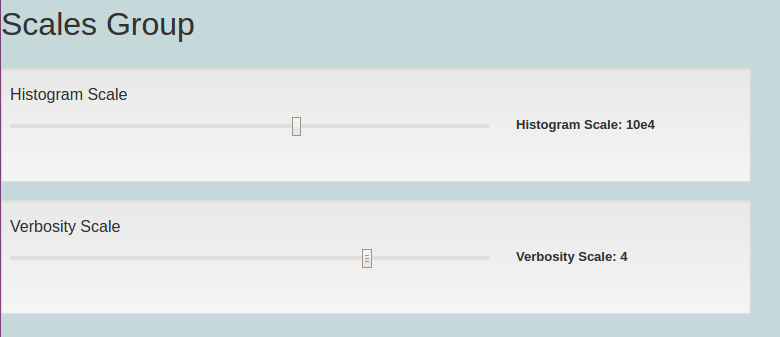
\includegraphics[scale=0.25]{ParticularScalesExpo.png} 
\caption{ Final version: an example of exponential scale (the first) followed by a non-exponential scale (the second) }
\end{figure}  

\newpage

Other setting are more easily accessible by some yes/no dropdown menus:


\begin{figure}[H]
\centering
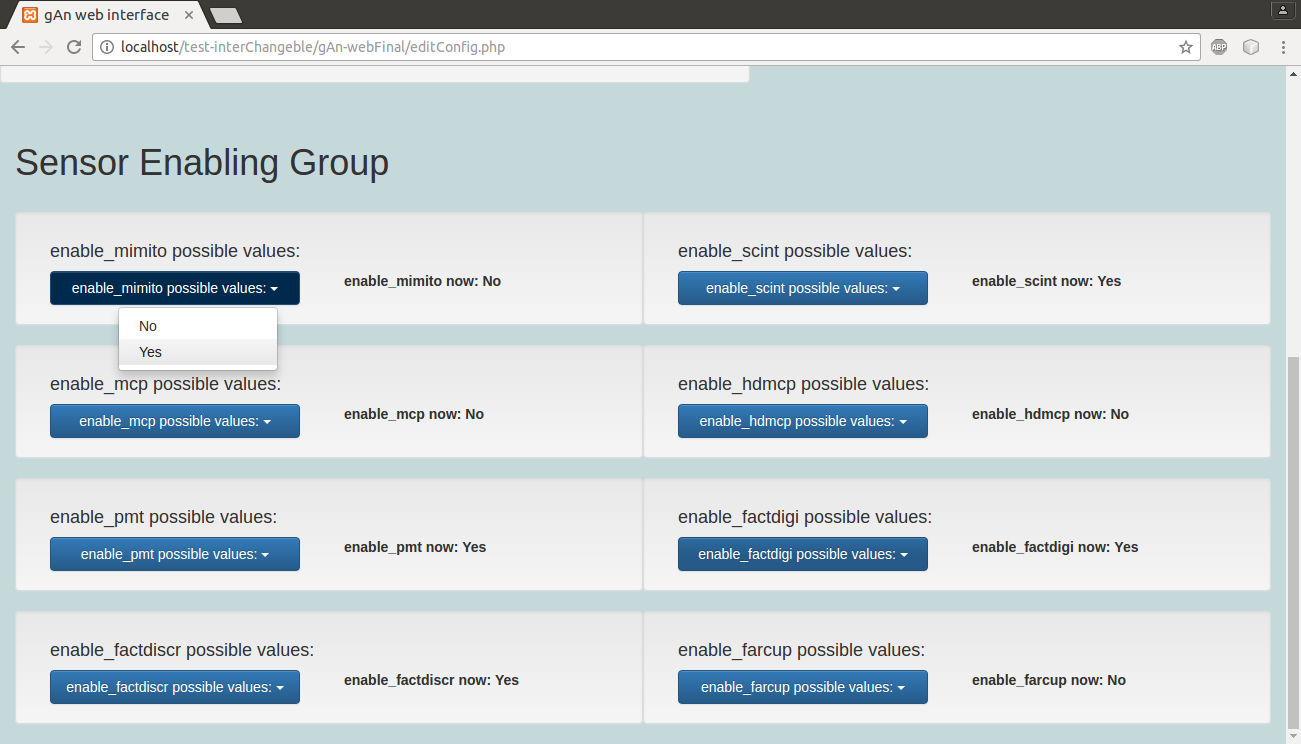
\includegraphics[scale=0.25]{ParticularYesNoConfig.png} 
\caption{ Final version: a group of dropdown menus }
\end{figure}  

\newpage

Output: 

There are some innovations. The first one is the navbar: now the user can find here all the most important commands. Before there was more buttons, distributed in the screen, and during the tests the users had problems to found them and to understand their functionalities. Now the navbar is more clear and organized:

\begin{figure}[H]
\centering
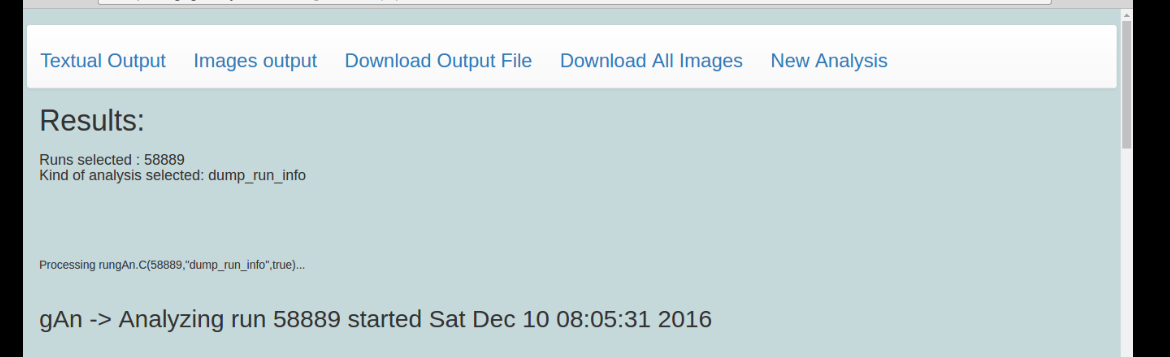
\includegraphics[scale=0.35]{LastNavbar.png} 
\caption{Final version: the Navbar}
\end{figure}  


Textual Output:

\begin{figure}[H]
\centering
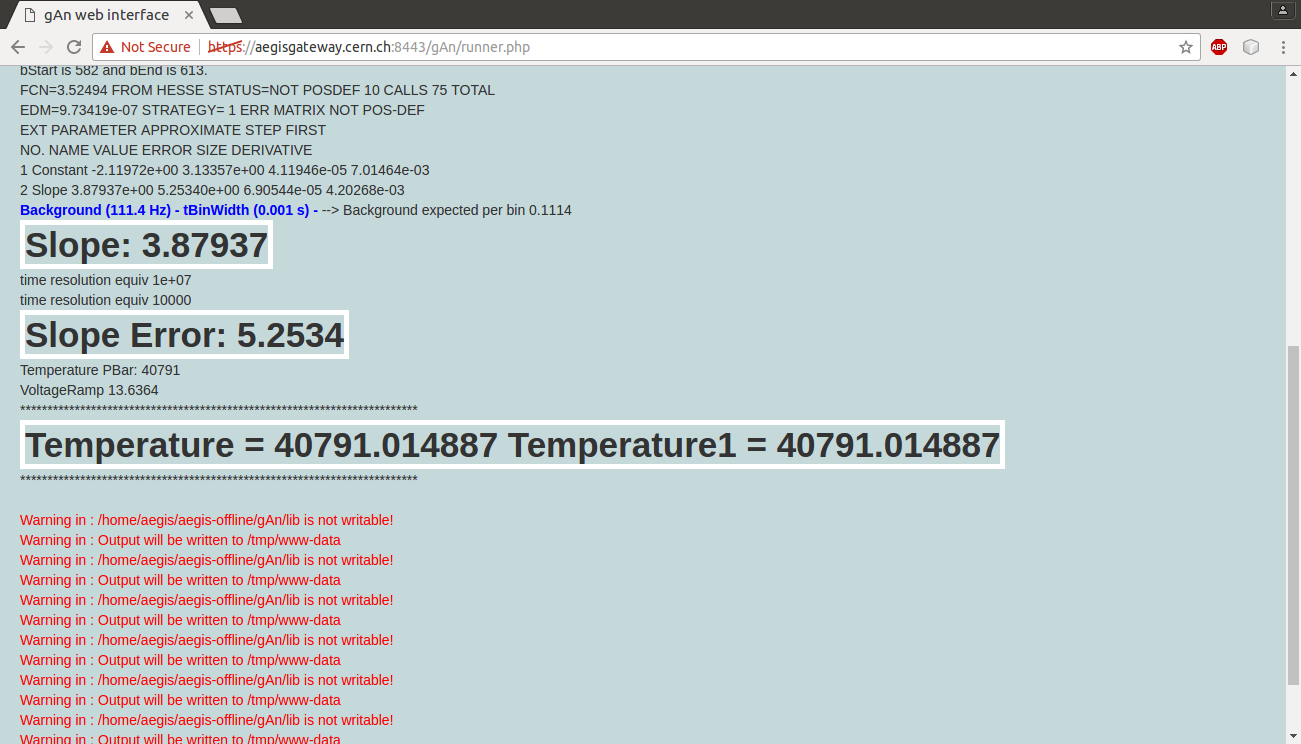
\includegraphics[scale=0.25]{LastTextualOutputHighLight.png} 
\caption{Final version: the output in textual version}
\end{figure}  

Here we can see out a textual output appears: there are more information, but in the 95 per cent of cases only a few are really useful, so they are highlighted with a special font and a big border (the hope is to use perceptive suggestions to advise the user about where to find what he searches). In this example we can see also some warnings: where something works wrong (or simply not perfectly) the system informs the user about the problem, with a red color, to ensure that he sees it. 

Let's make a confrontation between the same textual output before and after being formatted:

\begin{figure}[H]
\centering
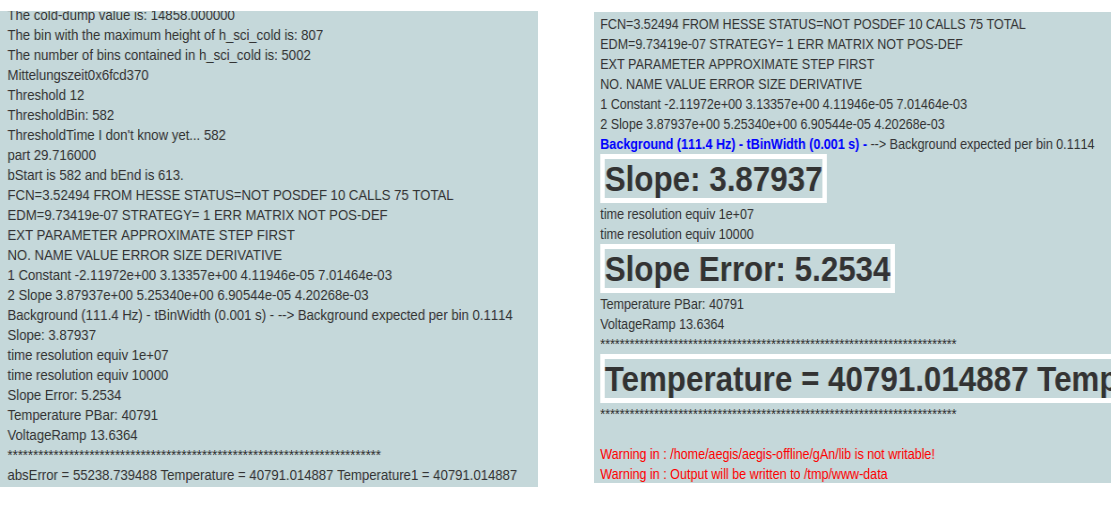
\includegraphics[scale=0.45]{TextConfrontation.png} 
\caption{Final version: formatted vs unformatted output}
\end{figure}  


Images output:

\begin{figure}[H]
\centering
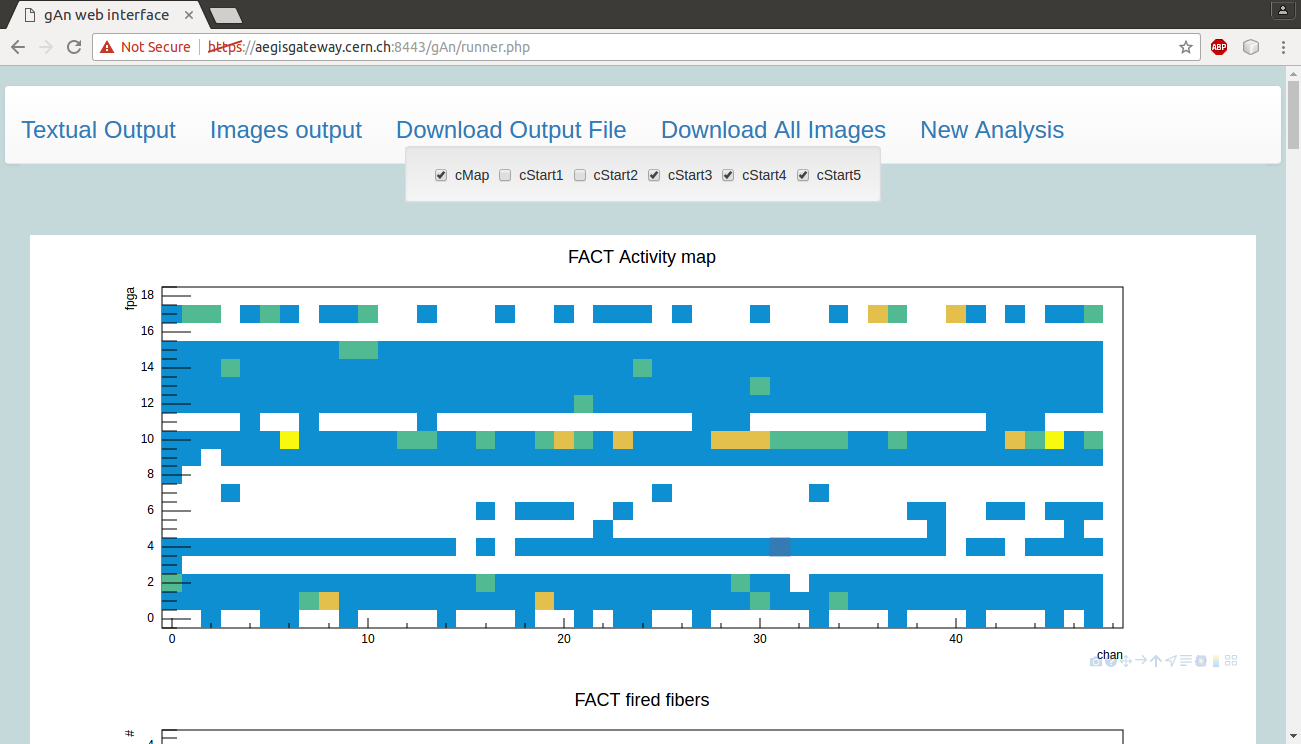
\includegraphics[scale=0.25]{ImageOutput.png} 
\caption{Final version: the output images}
\end{figure}  

Here we can see that there is no more the opportunity to select the dimension of the images (but still there is a zoom function in the image), or the layout, because none of the users never used these functionalities in the tests .. nor the possibility to choose a particular run of a group of images: this is because like discussed previous in this chapter the existing of the "kinds" of analysis makes this choice useless. Actually the navbar with these options is completely removed: the goal of this choice is to avoid the "information overload", so not to give the users too many commands and options, even more if these options are considered quite useless by the users.
Instead there is a list of check-boxes that if selected or deselected let the images appear and disappears. This feature is not determinant with 2 or 3 images, but sometimes the images are 7-8-9 so it is necessary.

\begin{figure}[H]
\centering
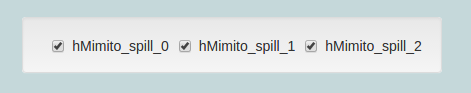
\includegraphics[scale=0.45]{ParticularHowToSelectImages.png} 
\caption{Final version: how the user can choose which images to show}
\end{figure}


An observation: sometimes the output is a list of images, vertically organized in a framework, some other times is a single image with more graph on a single sheets (a graph for each run inserted by the user as input, now all with the same color, but soon each run with a personal color); why?
The output is a single image on a single sheet when the goal is to compare different charts to see what is different, the output is an array of separate images when the goal is more related to the exploration, when the different images don't contain the same type of information. Sometimes is interesting make a confrontation between two images: in that case they are usually positioned horizontally. Who can decide what is the goal in each case? The solution is simple: who creates the analysis, so the back-end of this system codifies directly in the program how to show the charts in one or more sheets. This is because nobody better than who creates a particular analysis can understand what are the goals of this analysis.


\begin{figure}[H]
\centering
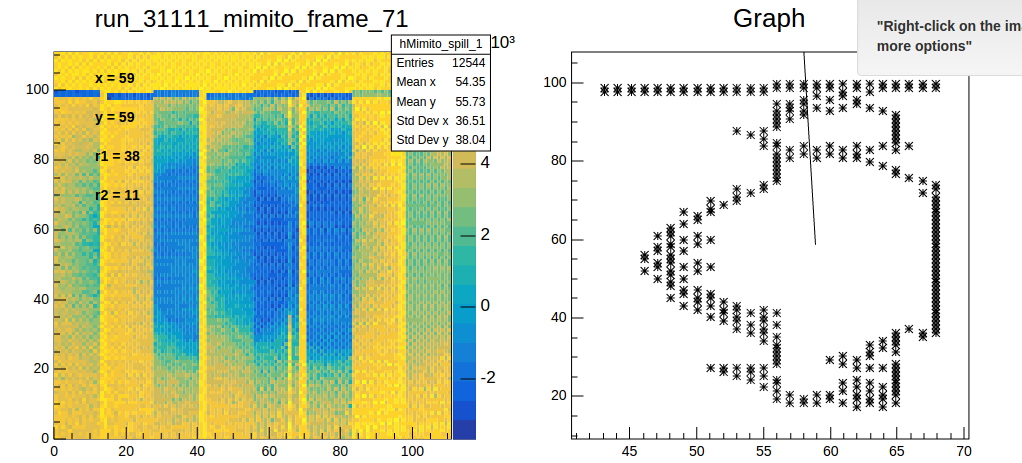
\includegraphics[scale=0.35]{ParticularConfrontationImages.png} 
\caption{Final version: Images that are meant to be compared}
\end{figure}   


Also in the "output image" case we observed that the users in most cases search in the images (almost) always the same information, so in some images the most important data (often they are dimension of peaks or integrals of spaces, or distances between peaks, or, in the case of charts with a time on the x-axis, auto-generated timelines about asynchronous events and triggers happened etc..) are directly written on the picture, like the following examples:

\begin{figure}[H]
\centering
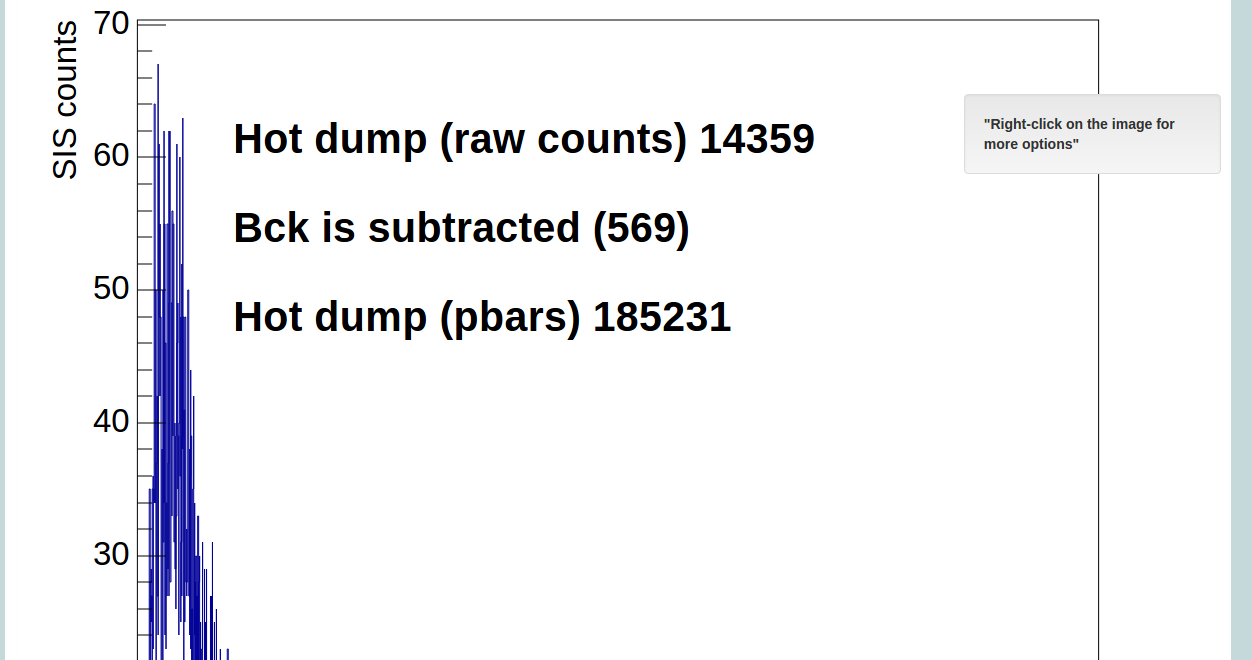
\includegraphics[scale=0.25]{LastImagenotes.png} 
\caption{Final version: images with info}
\end{figure}   

\begin{figure}[H]
\centering
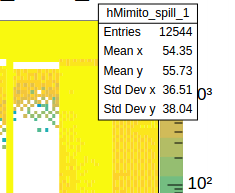
\includegraphics[scale=0.5]{ParticularFastReadInfos.png} 
\caption{Final version: other image with special info in a clear position }
\end{figure}   

There we can observe that the important information can be shown directly on the plot of the image (if they are graphical information, for example peaks, position of triggers etc) or in a special square on the top-right of the image (if they are not directly related to the image, but come from calculation or machine's settings).

\newpage

There is again the opportunity to access more information right clicking on the graph, of modifying it in various ways for example showing the graph in three dimensions: 

\begin{figure}[H]
\centering
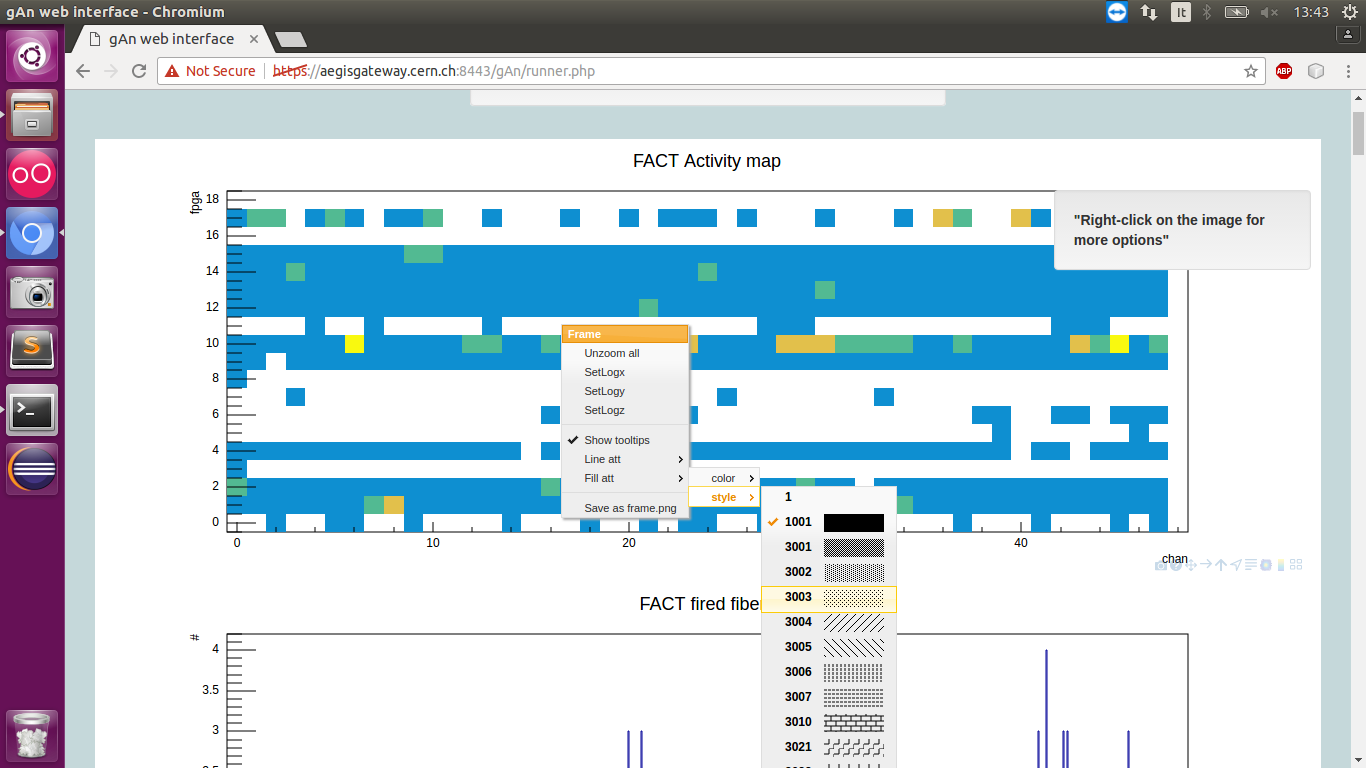
\includegraphics[scale=0.25]{LastImageOptions.png} 
\caption{Final version: some options}
\end{figure}  

\begin{figure}[H]
\centering
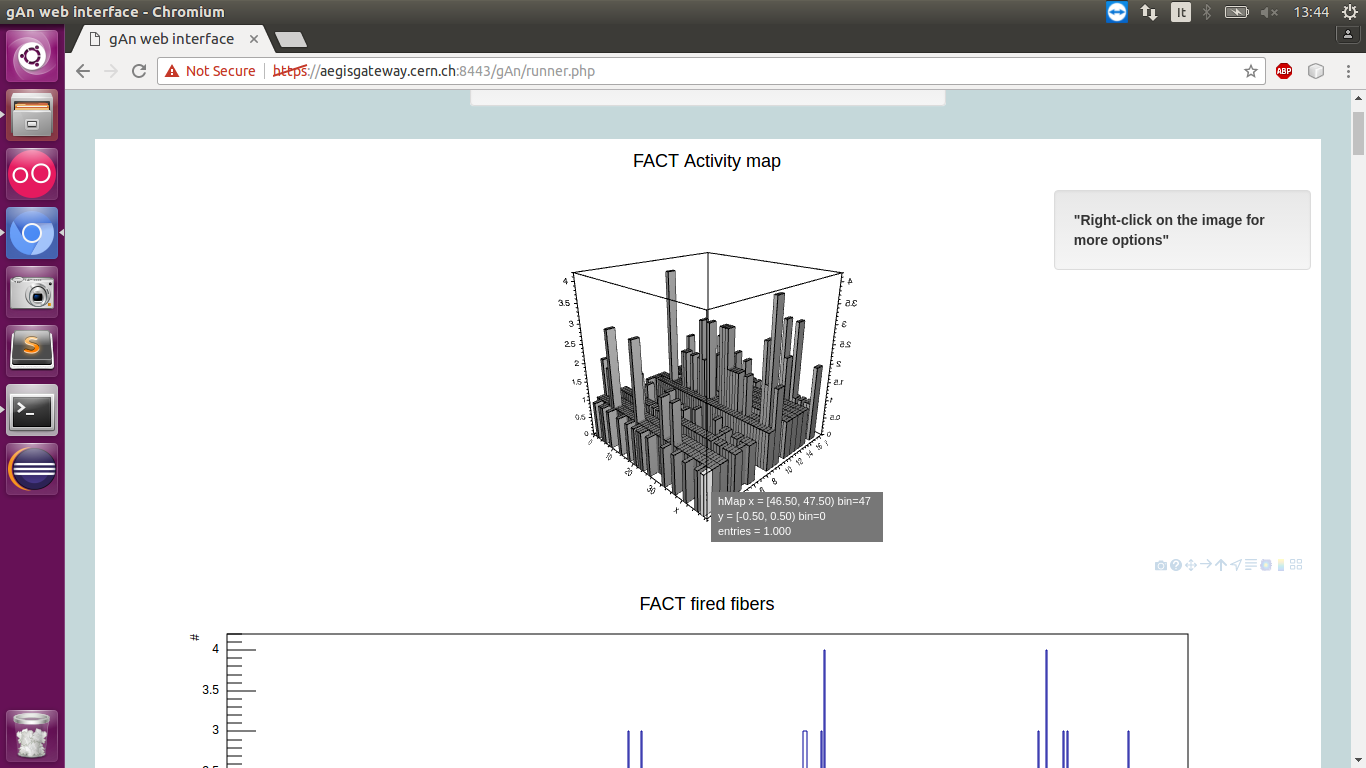
\includegraphics[scale=0.25]{LastGraphImage2.png} 
\caption{Final version: other option}
\end{figure}  

Often the users in the tests had problems understanding that with a right click they could access these functionalities, so now there is a specific label on the right of the screen to inform them (this label is in fixed position, but became visible only if the user arrive with the scrollbar on the images):

\begin{figure}[H]
\centering
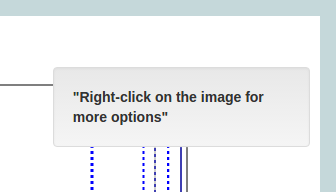
\includegraphics[scale=0.45]{LastImageLabel.png} 
\caption{Final version: label to inform the user about a feature}
\end{figure} 

There are some additional commands, that actually nobody used in the tests. Having on the screen commands that nobody uses is a potential source of confusion, but the developer is not absolutely sure about the idea of delete them. A good solution is to have them in the bottom of the frame of the image, not very highlighted, because they are not very important. Probably in a future confrontation with the super-users (is important to remember that this stage is never finished and always open to modification) these commands will be deleted.
They are in the following image:

\begin{figure}[H]
\centering

\includegraphics[scale=0.45]{ParticularUnusedControls.png} 
\caption{Final version: not frequently used controls}
\end{figure}  